% This work is licensed under the Creative Commons
% Attribution-NonCommercial-ShareAlike 4.0 International License. To view a copy
% of this license, visit http://creativecommons.org/licenses/by-nc-sa/4.0/ or
% send a letter to Creative Commons, PO Box 1866, Mountain View, CA 94042, USA.



\tikzset{every picture/.style={line width=0.75pt}} %set default line width to 0.75pt        

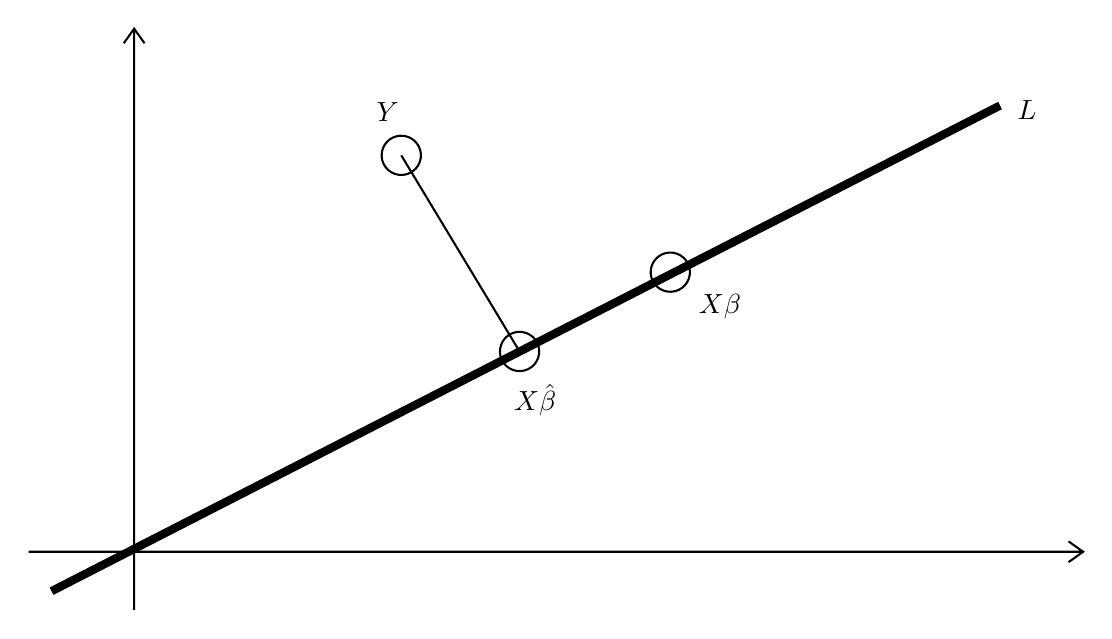
\begin{tikzpicture}[x=0.75pt,y=0.75pt,yscale=-1,xscale=1]
%uncomment if require: \path (0,300); %set diagram left start at 0, and has height of 300

%Shape: Axis 2D [id:dp7098119764904821] 
\draw  (50,256.93) -- (558,256.93)(100.8,4.93) -- (100.8,284.93) (551,251.93) -- (558,256.93) -- (551,261.93) (95.8,11.93) -- (100.8,4.93) -- (105.8,11.93)  ;
%Straight Lines [id:da9071558730776327] 
\draw [line width=3]    (61,275.93) -- (518,41.93) ;


%Straight Lines [id:da7398348018165936] 
\draw    (210,68.93) ;


%Straight Lines [id:da721943207149605] 
\draw    (229.5,65.93) -- (286.5,160.43) ;


%Shape: Circle [id:dp22369371272099947] 
\draw   (277.13,159.1) .. controls (277.87,153.92) and (282.66,150.33) .. (287.84,151.07) .. controls (293.01,151.81) and (296.61,156.6) .. (295.87,161.77) .. controls (295.13,166.94) and (290.34,170.54) .. (285.16,169.8) .. controls (279.99,169.06) and (276.39,164.27) .. (277.13,159.1) -- cycle ;
%Shape: Circle [id:dp5421173957527967] 
\draw   (349.75,120.88) .. controls (350.49,115.71) and (355.28,112.12) .. (360.45,112.86) .. controls (365.63,113.59) and (369.22,118.39) .. (368.48,123.56) .. controls (367.74,128.73) and (362.95,132.33) .. (357.78,131.59) .. controls (352.6,130.85) and (349.01,126.06) .. (349.75,120.88) -- cycle ;
%Shape: Circle [id:dp28472585647194326] 
\draw   (220.13,64.6) .. controls (220.87,59.42) and (225.66,55.83) .. (230.84,56.57) .. controls (236.01,57.31) and (239.61,62.1) .. (238.87,67.27) .. controls (238.13,72.44) and (233.34,76.04) .. (228.16,75.3) .. controls (222.99,74.56) and (219.39,69.77) .. (220.13,64.6) -- cycle ;

% Text Node
\draw (531,43.93) node  [align=left] {$L$};
% Text Node
\draw (223,44.93) node  [align=left] {$Y$};
% Text Node
\draw (294,183.93) node  [align=left] {$X\mal\hat{\beta}$};
% Text Node
\draw (383,138.93) node  [align=left] {$X\mal\beta$};


\end{tikzpicture}
